\subsection{\textbf{\uppercase{Implementação de Webservices no GSAN}}}

A estratégia de desenvolver o Webservice internamente ao sistema GSAN, foi adotada visando a possibilidade de reaproveitamento das regras de negócio, entidade, controlados dentre os demais artefatos que fazem parte do sistema.  Os novos serviços foram desenvolvidos sob tecnologias compatíveis com as utilizadas no sistema GSAN, utilizando a especificação JAX-WS\footnote{JAX-WS - \textit{Java API for XML-Based Web Services}}  para serem consumidos por sistemas externos através de submissões de arquivos do tipo XML, definidas no padrão de comunicação SOAP. Para tratar de conversões de arquivos XML para objetos e vice-versa está sendo utilizada a especificação do padrão JAXB\footnote{JAXB - \textit{Java Architecture for XML Binding}}, dessa forma estes serviços são executados no mesmo servidor de aplicação.
Na prática é necessário importar ao projeto as seguintes bibliotecas descritas abaixo;

% LIBS UTILIZADAS
 Prover suporte a configuração do End-Points (Serviços);
	\begin{itemize}
		\item jaxws-api-2.2.jar
		\item jaxws-rt.jar
		\item jaxws-tools.jar		
	\end{itemize}
	Fornecer suporte ao tratamento de serialização\footnote{Serialização refere-se ao processo de conversão de um objeto em bytes.} dos XML;
	\begin{itemize}
		\item jaxb-impl.jar
		\item jaxb-xjc.jar
		\item policy.jar
		\item stax-ex.jar
		\item stax2-api.jar
		\item streambuffer.jar
		\item woodstox-core-asl.jar		
	\end{itemize}


Após realizar a configuração das bibliotecas necessárias para implementação, foram definidos os seguintes novos serviços para automatizar os processos de Obtenção da 2ª via de conta, Informar Falta de Água e Solicitar Restabelecimento da Ligação;

\begin{description}
	\item \textbf{\textit{isOnline}}: Realiza verificação de disponibilidade do sistema.
	\item \textbf{\textit{pesquisarImovelOuCliente}}: Obtém detalhes sobre um imóvel ou cliente cadastro no sistema GSAN.
	\item \textbf{\textit{obter2ViaConta}}: Gerar a 2ª via de conta pendente.
	\item \textbf{\textit{informarFaltaAgua}}: Formalizar junto ao sistema GSAN um Registro de Atendimento do tipo Falta de Água.
	\item \textbf{\textit{solicitarRestabelecimento}}: Formalizar junto ao sistema GSAN um Registro de Atendimento do tipo Solicitar Restabelecimento da Ligação de Água.
\end{description}

A figura \ref{figura:interfaceServicosAutomatizados} abaixo, demonstra a declaração dos métodos do \textit{Webservice}.

\begin{figure}[H]
	\centering
	\caption{\textbf{Interface dos serviços automatizados.}}	
	\label{figura:interfaceServicosAutomatizados}
	\begin{subfigure}[H]{\textwidth}
		\centering
		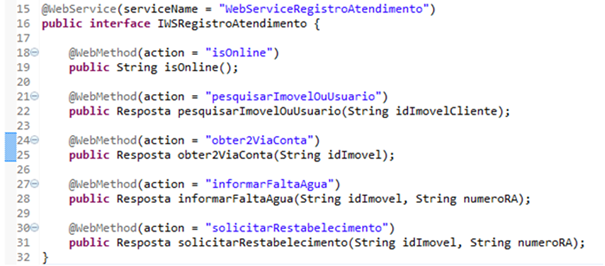
\includegraphics{figuras/implementacao_servicos.png}
		\legend {\fontsize{10}{12}\selectfont {Fonte: Autoria Própria}.}	
	\end{subfigure}
\end{figure}



Para definir a URL\footnote{URL - \textit{Uniform Resource Locator}} de acesso ao \textit{Webservice} será preciso atualizar o arquivo web.xml, declarando a servlet padrão definida na especificação do JAX-WS para esse propósito, conforme a figura \ref{figura:declaracaoServlet}:

\begin{figure}[H]
	\centering
	\caption{\textbf{Declaração da servlet do Webservice.}}	
	\label{figura:declaracaoServlet}
	\begin{subfigure}[H]{\textwidth}
		\centering
		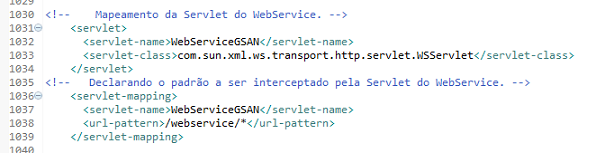
\includegraphics{figuras/declarando_servlet.png}
		\legend {\fontsize{10}{12}\selectfont {Fonte: Autoria Própria}.}	
	\end{subfigure}
\end{figure}

Feito isso, será preciso disponibilizar os novos serviços, definindo a Classe Concreta\footnote{Classe Concreta refere-se a classes que possuem atributos, métodos e construtores, passível de instanciação.} de implementação e o padrão de acesso que será adotado para a interface criada, para que as solicitações sejam interceptadas adequadamente redirecionadas ao \textit{EndPoints} corretos, com isso será necessário criar o arquivo com a seguinte nomenclatura \textit{sun-jaxws.xml}, localizado dentro do diretório WEB\_INF da aplicação, segue abaixo o conteúdo do arquivo, conforme a figura \ref{figura:declaracaoEndPoint}:

\begin{figure}[H]
	\centering
	\caption{\textbf{Declaração do \textit{EndPoint} dos serviços.}}	
	\label{figura:declaracaoEndPoint}
	\begin{subfigure}[H]{\textwidth}
		\centering
		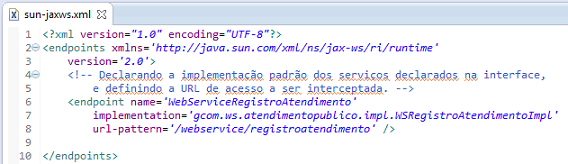
\includegraphics{figuras/declaracao_endpoint.png}
		\legend {\fontsize{10}{12}\selectfont {Fonte: Autoria Própria}.}
	\end{subfigure}
\end{figure}


Realizado todos esses passos o sistema GSAN conseguirá disponibilizar os novos serviços declarados na interface de Registro de Atendimento, dessa forma o acesso será realizado da seguinte maneira:

\begin{description}
	\item htttp://<servidor>:<porta>/gsan/webservice/registroatendimento
\end{description}

Estando apto a ser integrado com sistemas externos. 